\renewcommand{\relPath}{SECTION/40_Pulsing/}
 
\chapter[Pulsed Excitation Measurement]{Measuring the effects of a pulsed 
  excitation on the build up of acoustic streaming and the acoustic radiation 
  force utilizing an optical tweezer
}\label{ch:pulsing}
\textit{This chapter is original work by Christoph Goering:
\footnote{: DOI: 10.1103/PhysRevE.104.025104, reproduced under the terms of the 
Creative Commons Attribution 4.0 license.}}

\vspace{5mm} \noindent
C. Goering and J. Dual, "Dynamic measurement of the acoustic streaming time 
constant utilizing an optical tweezer", Physical Review E, 2021, \textbf{104}, 
025104.


\section{Abstract}

Pulsed excitations of piezoelectric transducers affect during the build up the 
force contributions from acoustic streaming (AS) and the acoustic radiation 
force (ARF) to the total force in a standing pressure wave differently. We find 
with an optical tweezer as measuring instrument that during the first 120'000 
excitation periods and across different pulsing frequencies, the AS induced 
displacement is in average less than 20\% of its non-pulsed value for a duty 
cycle of 50\%, whereas the ARF induced displacement is around 50\%. These 
findings show that a pulsed excitation can be a tool for reducing AS compared 
to the ARF.

%%%%%%%%%%%%%%%%%%%%%%%%%%%%%%%%%%%%%%%%%%%%%%%%%%%%%%%%%%%%%%%%%%%%%%%%%%%%%%
\section{Introduction}

In acoustofluidic devices two main forces lead to a displacement of an immersed 
object within a pressure wave field: the drag force from acoustic streaming 
(AS) and the acoustic radiation force (ARF). AS typically arises due to viscous 
losses. These viscous losses can appear in the fluid itself (Eckart type 
streaming) \cite{Eckart1948} or in a viscous boundary layer. This boundary 
layer can either be at the interface between the fluid cavity and the 
surrounding medium (Schlichting and Rayleigh streaming) 
\cite{Nyborg1965,Schlichting1932} or even around the object itself 
(microstreaming) \cite{Baasch2019}. Apart from microstreaming, the occurrence 
of AS is independent of the immersed object properties.

The other main force is the ARF. As AS, it is a second order time-averaged 
effect and appears due to scattering of the acoustic incident field at the 
object surface \cite{Yosioka1955,Bruus2012,Gorkov1962}. In contrast to AS, the 
ARF depends also on the ratios of the object and fluid material. For example, 
an object of any material but with an acoustic contrast factor $\Phi$ 
\cite{Bruus2012} of zero magnitude is not displaced due to the ARF because the 
ARF scales linearly with $\Phi$. However, this object will be displaced by the 
drag force arising from AS for any value of $\Phi$.

Besides the material influence, another important difference is the scaling 
with the object dimension for the limit of small particles compared to the 
acoustic wavelength \cite{Bruus2012,King1934}. On the one hand, the drag force 
from AS scales for a spherical object with the radius ($\FAS\propto \R$), and 
on the other hand, the ARF scales with the object volume ($\FARF\propto 
\R^{3}$) \cite{Bruus2012}. At the critical radius ($\R=\Rcrit$) both forces are 
equal in magnitude ($\FARF=\FAS$). For a radius smaller than the critical 
radius ($\R<\Rcrit$) \cite{Bruus2012,Barnkob2012} the drag force from AS 
dominates over the ARF and vice-versa. The forces from AS can be neglected if 
$\R\gg\Rcrit$.

In many acoustofluidic applications the drag forces from AS are undesired 
because they can counteract the ARF \cite{VanAssche2020,Antfolk2014} and hinder 
the application's desired function, e.g. the trapping or focusing of particles. 
Therefore, different techniques for the suppression of AS have been 
investigated in recent years. Hoyos and Castro applied a pulsed excitation to 
the piezoelectric transducer (PZT) leading to a reduction of the steady-state 
streaming flow of up to 50\% compared to the unpulsed flow 
\cite{Hoyos2013,Castro2016}.  \cname{Karlsen2018a} utilized in simulations and 
experiments inhomogeneities of the density and of the compressibility within 
the fluid to reduce AS. \cname{Bach2020} optimized the shape of channels with 
numerical simulations to reduce AS by two orders of magnitudes while retaining 
the same level of acoustic pressure. The same AS suppression magnitude was 
achieved by \cname{Winckelmann2021}. They investigated analytically and 
numerically the usage of acoustic electroosmosis to suppress AS.

The combination of optical tweezer (OT) and the acoustic trap is relatively new 
and rare. To the best of the authors' knowledge, \cname{Thalhammer2011} were 
\citeyear{Thalhammer2011} the first to combine these two kind of traps to 
measure the acoustic forces with the OT. In 2014, \cname{Bassindale2014} 
utilized an holographic OT to measure acoustic forces in three dimensions, and 
\cname{Fury2014} used the fine spatial optical resolution and the wide range of 
acoustic trapping for spatially precise manipulation of microbubbles. In 2015 
and 2016, \cname{Lakaemper2015} and \cname{Lamprecht2016} used our single beam 
optical trap to measure the acoustic forces in two and tree dimensions on 
silica micro particles. In 2016, \cname{Thalhammer2016} also combined a 
holographic OT with an acoustic trap to measure the force for excitation 
frequencies above \SI{20}{\mega\hertz}. Lastly in 2021, \cname{Lamprecht2021} 
used our setup to measure the resulting final rotational velocity on 
microparticles due to the acoustic viscous torque.

In 2021, we~\cite{Goering2021} used an OT setup to measure for the first time 
the build up of the ARF and AS on a single spherical particle in a precisely 
characterized \si{\mega\hertz} pressure field. We found that the build up of AS 
is much slower than the build up of the ARF. Our measurements of the AS build 
up revealed approximately 4 times longer build up of AS than the theoretical 
prediction from the momentum diffusion time approximation 
\cite{Muller2015,Goering2021}. Those experimental results indicated that the 
longer-than-expected build up of the AS might be the reason for the pulsed 
excitation to successfully suppress the AS \cite{Hoyos2013,Castro2016}.

Here, we use our measurement routine, the OT setup, the acoustofluidic bulk 
acoustic wave device, and the same acoustic excitation frequency from 
\cite{Goering2021} to dynamically measure the build up of the ARF and AS for a 
acoustic excitation with various pulsing parameter settings.

%%%%%%%%%%%%%%%%%%%%%%%%%%%%%%%%%%%%%%%%%%%%%%%%%%%%%%%%%%%%%%%%%%%%%%%%%%%%%%

%%%%%%%%%%%%%%%%%%%%%%%%%%%%%%%%%%%%%%%%%%%%%%%%%%%%%%%%%%%%%%%%%%%%%%%%%%%%%%
\section{Measurement Protocol}

\begin{figure}[tbp]
  \centering
  % \tikzsetnextfilename{PU-device}
{
\tiny

\begin{tikzpicture}
  % lens
  \definecolor{tempcolor}{RGB}{222, 201, 84}
  \draw[color=white,fill=tempcolor] (0,0.5) circle (0.8);

  % R = (0.2^2+0.4^2)/2/0.2 = 0.5
  % alpha = arcsin(0.4/R) ~53 deg
  \definecolor{tempcolor}{RGB}{176, 206, 255}
  \filldraw[color=black, fill=tempcolor, ultra thin] (-0.4,1) arc 
  (217:323:0.5);

  \draw[fill=white] (-0.5,1) rectangle ++(1,2);

  % PZT
  \filldraw[black,pattern=north west lines] (-3.5,0.7) rectangle ++(0.7,0.2);

  % SI
  \filldraw[black] (-3,-0.5) rectangle ++(-0.5,1);
  \filldraw[black] (+3,-0.5) rectangle ++(+0.5,1);

  % Glas
  \filldraw[color=black, fill=black!15, ultra thin] (-3.5,0.5) rectangle 
  ++(7,0.2);
  \filldraw[color=black, fill=black!15, ultra thin] (-3.5,-0.5) rectangle 
  ++(7,-0.4);

  \draw[|<->|] (-3.5, -1.1) -- node[pos=0.18, below] {\SI{26}{\mm} 
  ($L=\SI{76}{\mm}$)} ++(7,0);

  % cavity
  \filldraw[color=black, fill=blue!20, ultra thin] (-3,-0.5) rectangle ++(6,1);
  \draw[|<->|] (-3, -0.6) -- node[pos=0.2, below] {\SI{3}{\mm}} ++(6,0);
  \draw[|<->|] (-2.8, -0.5) -- node[pos=0.15, right] {\SI{0.1}{\mm}} ++(0,1);

  %pressure field
  \draw[white, variable=\x, domain=-3:3, samples=500] (-1,0) plot 
  (\x,{cos(\x*pi r*3)/4});
  \draw[white, variable=\x, domain=-3:3, samples=500] (-1,0) plot 
  (\x,{-cos(\x*pi r*3)/4});
  % \node at (-2,0.4) {\textcolor{white}{$p_{\mathrm{a}}$}};

  % coordinate system
  \draw[->] (0,0) -- node[pos=1, right] {$\bm{e}_{y}$} ++(0.7,0);
  \draw[->] (0,0) -- node[pos=1, above] {$\bm{e}_{z}$} ++(0,1.7);

  % particle
  \shade[ball color=black!5] (0,0) circle (0.2);

  % condensor
  \filldraw[tempcolor] (0,-1.5) ellipse (1.4 and 0.2);

  % laser
  % \draw[red] (0.35,3.1) -- (0.35,0.92) -- (0,0);
  \draw[red] (0.35,3.1) -- (0.35,0.92) -- (-0.57,-1.5) -- ++(0,-0.3);
  \draw[red] (-0.35,3.1) -- (-0.35,0.92) -- (0.57,-1.5) -- ++(0,-0.3);

  % annotations
  \node[above, align=right, text width=35mm] at (-2.5, 0.9) {PZT 
  (\SI[product-units = single]{4 x 0.5 x 20}{\mm})};
  \node[right] at (1.4, 0.35) {Cavity};
  \node[right] at (1.4, -1.5) {Condensor lens};

  \draw[ultra thin] (0.55, 0.8) -- node[pos=1, right] {Immmersion layer} 
  (1.4,0.9);

  \draw[ultra thin] (0.2, 0.9) -- node[pos=1, right] {Focussing lens} 
  (1.4,1.3);


\end{tikzpicture}
}

  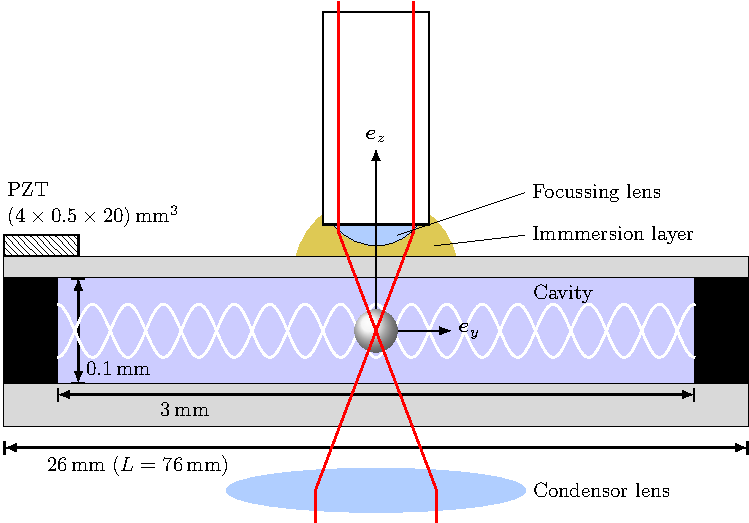
\includegraphics[width=120mm]{External/PU-device.pdf}
  \caption{Schematic of device and build up measurement 
  setup.}\label{fig:PU-device}
\end{figure}

We will highlight the main points of the measurement protocol for the build up 
measurements (BM). A more extensive explanation of each step can be found in 
\citeauthor{Goering2021} \cite{Goering2021}. We can measure with the OT the 
build up of the ARF and AS separately because we determined our BM locations 
such that those two effects are orthogonal to each other; i.e., the ARF points 
in the direction of our $y$ coordinate and the AS points along $z$ (see 
\cref{fig:PU-device}). Our setup (see \cref{fig:PU-protocol}; see also [supplemental 
material] for more detailed figures of the OT and the used device) has in its 
back focal plane two quadrant photo detectors (QPDs) for detecting the movement 
in each spatial direction separately 
\cite{Lakaemper2015,Goering2021,Lamprecht2021,Lamprecht2016}. One QPD measures 
the information of the $x$ and $y$ coordinate and the other QPD measures the 
$z$ information. Hence, the build up information of the ARF and AS are also 
separated in the data.

\begin{figure*}[tbp]
  \centering
  % \tikzsetnextfilename{PU-protocol}
{
  \tiny
  \definecolor{tempcolor}{RGB}{176, 206, 255}
\begin{tikzpicture}

% close shutter
\def\y{0}
\pgfmathsetmacro{\ybottom}{\y-0.25)}
\pgfmathsetmacro{\ytop}{\y+0.25)}
\pgfmathsetmacro{\yshutter}{\y-0.5)}
\pgfmathsetmacro{\yshuttert}{\y+0.5)}
\pgfmathsetmacro{\qpd}{\y-0.4)}
\pgfmathsetmacro{\tlaser}{\y+0.2)}
\pgfmathsetmacro{\blaser}{\y-0.2)}
\pgfmathsetmacro{\power}{\y+1.2)}

  \draw[black] (0,\ybottom) rectangle ++(1,0.5);
  \path (0,\ytop) -- ++(1,0) node[above, midway, anchor=south] {Laser};

  \fill[tempcolor] (2.5,\y) ellipse (0.15 and 0.75);
  \path (2,0.75) -- ++(1,0) node[above, midway, anchor=south] {Focussing lens};

  \shade[ball color=black!10] (3.5,\y) circle (.25);

  \path (3.25,\ytop) -- ++(0.5,0) node[above, midway] {particle};
  \path (3.25,\ybottom) -- ++(0.5,0) node[below, midway] {trapped};

  \fill[tempcolor] (4.5,\y) ellipse (0.15 and 0.75);
  \path (4,0.75) -- ++(1,0) node[above, midway, anchor=south] {Condensor lens};

  \filldraw[color=black, fill=black!50] (5.5,\yshutter) rectangle ++(1,1);
  \path (5.5,\yshuttert) -- ++(1,0) node[above, midway, anchor=south] 
  {shutter};
  \path (5.5,\y) -- ++(1,0) node[midway] {$T< 1\%$};
  \path (5.5,\yshutter) -- ++(1,0) node[below, midway] {closed};

  \fill[tempcolor] (7.5,\y) ellipse (0.15 and 0.75);
  \path (7,0.75) -- ++(1,0) node[above, midway, anchor=south] {lens 3};

  \filldraw[color=black, fill=black!10] (9,\qpd) rectangle ++(0.8,0.8);
  \path (9,0.5) -- ++(0.8,0) node[above, midway, anchor=south] {QPDs};
  \filldraw[color=red!50] (9.4,\y) circle (.2);

  \draw[dotted, black] (9, \y) -- ++(0.8,0);
  \draw[dotted, black] (9.4, \qpd) -- ++(0,0.8);

  \draw[red, thick] (1,\blaser) -- ++(1.5,0) -- ++(2,0.4) -- (5.5,\tlaser);
  \draw[red, thick] (1,\tlaser) -- ++(1.5,0) -- ++(2,-0.4) -- (5.5,\blaser);
  \draw[red!50, thick, dashed]  (6.5,\tlaser) -- ++(1.0,0) -- (9.4,\blaser);
  \draw[red!50, thick, dashed]  (6.5,\blaser) -- ++(1.0,0) -- (9.4,\tlaser);

  \draw[black, |<->|] (1,\power) -- node[midway, above] {$P\approx 
  \SI{140}{\milli\watt}$} ++(5,0);

  \draw[black, <->|] (6,\power) -- node[midway, above] {$P<
  \SI{1}{\milli\watt}$} ++(3.4,0);
% open shutter
  \def\y{-2.5}
\pgfmathsetmacro{\ybottom}{\y-0.25)}
\pgfmathsetmacro{\ytop}{\y+0.25)}
\pgfmathsetmacro{\yshutter}{\y-0.5)}
\pgfmathsetmacro{\yshuttert}{\y+0.5)}
\pgfmathsetmacro{\qpd}{\y-0.4)}
\pgfmathsetmacro{\tlaser}{\y+0.2)}
\pgfmathsetmacro{\blaser}{\y-0.2)}
\pgfmathsetmacro{\power}{\y+0.9)}

  \draw[black] (0,\ybottom) rectangle ++(1,0.5);

  \fill[tempcolor] (2.5,\y) ellipse (0.15 and 0.75);

  \shade[ball color=black!10] (3.5,\y) circle (.25);
  \draw[color=red, -stealth, ultra thick] (3.5,\y) -- node[pos = 0.7,left] 
  {$F_{\mathrm{ac}}$} ++(0.55, 0.65);

  \path (3.25,\ybottom) -- ++(0.5,0) node[below, midway] {floating};

  \fill[tempcolor] (4.5,\y) ellipse (0.15 and 0.75);

  \filldraw[color=black, fill=black!10] (5.5,\yshutter) rectangle ++(1,1);
  \path (5.5,\y) -- ++(1,0) node[midway] {$T\approx 30\%$};
  \path (5.5,\yshutter) -- ++(1,0) node[below, midway] {open};

  \fill[tempcolor] (7.5,\y) ellipse (0.15 and 0.75);

  \filldraw[color=black, fill=black!10] (9,\qpd) rectangle ++(0.8,0.8);
  \filldraw[color=red!15] (9.4,\y) circle (.2);

  \draw[dotted, black] (9, \y) -- ++(0.8,0);
  \draw[dotted, black] (9.4, \qpd) -- ++(0,0.8);

  \draw[red!50, thick] (1,\blaser) -- ++(1.5,0) -- ++(2,0.4) -- (5.5,\tlaser);
  \draw[red!50, thick] (1,\tlaser) -- ++(1.5,0) -- ++(2,-0.4) -- (5.5,\blaser);
  \draw[red!15, thick, dashed]  (6.5,\tlaser) -- ++(1.0,0) -- (9.4,\blaser);
  \draw[red!15, thick, dashed]  (6.5,\blaser) -- ++(1.0,0) -- (9.4,\tlaser);

  \draw[black, |<->|] (1,\power) -- node[midway, above] {$P\approx 
  \SI{0.4}{\milli\watt}$} ++(5,0);

  \draw[black, <->|] (6,\power) -- node[midway, above] {$P<
  \SI{0.15}{\milli\watt}$} ++(3.4,0);


  %%% time axis
  \draw[|<->|,white] (-0.2,1) -- node[midway,rotate=90, above,align=center,text 
  width = 20mm,color=black] {before/after\\ measurement} ++(0,-2);

  \draw[|<->|,white] (-0.2,-1.5) -- node[midway,rotate=90, 
  above,align=center,text width = 20mm,color=black] {during\\ measurement} 
  ++(0,-2);

% dividing line
  \draw[black, ultra thick] (-1,-1.15) -- ++(11.4,0);
  \draw[black, dotted, thick] (-0.2,1.3) -- (-0.2,-3.5);
\end{tikzpicture}
}


  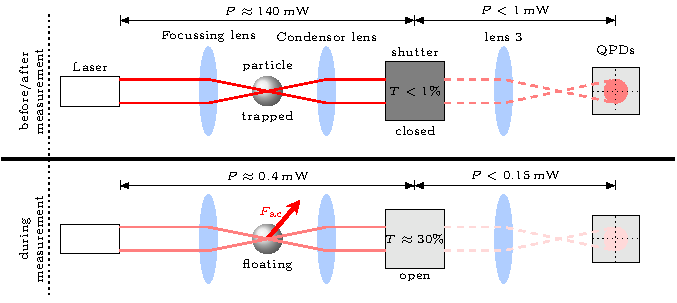
\includegraphics[width=\textwidth]{External/PU-protocol.pdf}
  \caption{Schematic of optical trapping setup, laser settings ($P$: laser 
    power), and optical shutter settings ($T$: transmittance for $\llaser = 
    \SI{785}{\nm}$) before and after the build up measurement (BM; top) and 
    during the BM (bottom). During the BM the particle is free floating, the 
    laser power is reduced as low as possible, the shutter is opened to allow 
    optical position detection on the quadrant photo detectors (QPDs), and the 
    ultrasound is switched on; hence there acts an acoustic force 
    $F_{\mathrm{ac}}$ on the particle. Before and after the BM all states are 
switched to their respective opposite.}\label{fig:PU-protocol}
\end{figure*}

Our OT consists of a single laser with a maximal power of \SI{200}{\milli\watt} 
and a wavelength of $\llaser = \SI{785}{\nm}$ (Omicron GmbH, Rodgau, Germany). 
The laser traps a spherical \SiO~particle with a radius of $R=\SI{1.03}{\um}$ 
(Microparticle GmbH, Berlin, Germany; same as in \cite{Goering2021}) and acts 
also as the light source for the displacement signal on the QPDs (see 
\cref{fig:PU-protocol}). In the normal trapping mode it is not possible to 
measure the build up of AS and the ARF because the timeconstant of the OT 
($\tau_{\mathrm{OT}}\approx \SI{1.59}{\ms}$ \cite{Goering2021}) is much larger 
than the ones of interest ($\tau_{\mathrm{AS}}\approx \SI{1.44}{\ms}$ and 
$\tau_{\mathrm{ARF}}\approx \SI{1.4}{\us}$ \cite{Goering2021}).  
$\tau_{\mathrm{ARF}}$ is defined as the build up time of the ARF, which is 
approximated by the build up time $\tau$ of a single degree of freedom acoustic 
resonance mode with quality factor $Q\approx 40$ and $\tau_{\mathrm{AS}}$ is 
the momentum diffusion time~\cite{Muller2015}. Therefore, we need to switch the 
laser almost completely off such that the formerly stably trapped particle 
becomes free-floating. If the particle is free-floating, there is no influence 
from the OT characteristics on the BM.

For stable trapping of our particles the laser power must be greater than at 
least \SI{75}{\milli\watt}. However, this laser intensity is too high for the 
QPDs in the back focal plane and they would be damaged without further 
modifications. Therefore, an optical shutter (FOS NIR 1100, LC-TEC, Borlänge, 
Sweden) is installed in the laser path before the QPDs (see 
\cref{fig:PU-protocol}). The shutter transmittance $T$ is proportional to the 
applied voltage of the shutter driving signal. In earlier experiments with our 
OT the optical shutter was implemented as a fixed set of neutral density 
filters that limited the transmitted intensity to less than 0.1\% of the 
trapping intensity \cite{Lakaemper2015,Lamprecht2016,Lamprecht2021}. Before and 
after our BMs the particle is stably trapped.

One single BM follows the sketched process of \cref{fig:PU-flowchart} (see also 
\cref{fig:PU-protocol}). The particle is free floating during the BM and 
re-trapped at the end. The spot size of the OT is not finite and re-trapping to 
the exact same location unlikely. Therefore at the beginning of each BM the 
Python control software checks if the offset of the QPDs needs to be adjusted. 
A QPD with zero offset is in the middle of the linear regime between the 
displacement of the particle and the measured voltage at the QPDs. Hence, the 
offset adjustment before a new BM enables the quantitative comparison between 
BMs because all begin with the same offset. If an adjustment is necessary, an 
automated incremental offset change is performed and the QPD values are checked 
again. If there is no action needed, the laser changes its power $P$ from 
\SI{140}{\milli\watt} to \SI{0.4}{\milli\watt} and the shutter starts to open. 
The laser power change takes effect in less than \SI{3}{\ms}, whereas the 
shutter is specified to open within \SI{15}{\ms} from fully closed to 90\% of 
its fully open state. To ensure the shutter is maximally opened we wait another 
\SI{10}{\ms} before the ultrasound (US) is switched on. In this first 
\SI{25}{\ms} ($t=\SI{-25}{\ms}$ to $t=\SI{0}{\ms}$) the particle is free 
floating and will therefore start sedimenting. We showed in \cite{Goering2021} 
that the particle travels less than $\SI{0.052}{\um}\approx 0.05\,R$ in this 
time towards the bottom of the device. This distance is uncritical for the 
further BM. At $t=\SI{0}{\ms}$ the US is switched on for \SI{30}{\ms}. The 
particle is displaced due to the acoustic forces $F_{\mathrm{ac}}$. At 
$t=\SI{55}{\ms}$, the shutter starts closing and the laser power is increased 
to its starting power again to retrap the same free-floating particle. After 
the output of the data a new BM starts. The time between two consecutive BMs 
is more than \SI{2}{\s}. The data for one BM is collected over a timespan of 
\SI{100}{\ms} where the US is switched on for \SI{30}{\ms} only. The acoustic 
excitation frequency $\fex$ is set to the same value of \SI{4.015}{\mega\hertz} 
where we measured 17 standing pressure nodal planes. With a maximal force 
amplitude of \SI{1.25}{\pico\newton} for a \SI{4.39}{\um} diameter particle and 
a maximal force amplitude of \SI{0.17}{\pico\newton} for a \SI{2.06}{\um} 
diameter particle (both measured with the OT~\cite{Goering2021}) and the 
assumption of an one dimensional pressure wave the acoustic pressure (see 
equations (30a) through (30c) in~\cite{Bruus2012}) inside the fluid cavity is 
about \SI{100}{\kilo\pascal}~\cite{Goering2021}. With this short time of US 
excitation and the fast build up constant for the ARF 
($\tau_{\mathrm{ARF}}\approx \SI{1.4}{\us}$) compared to the relatively long 
time between BMs, the system has the same starting conditions for each BM 
respectively.

\begin{figure*}[tbp]
  \centering
  % \tikzsetnextfilename{flowchart}
{
  \footnotesize

\begin{tikzpicture}[node distance=1cm]

  \node (start) [startstop] {Start\\[-3.5mm] measurement};
  \node (qpd) [io, right of=start, xshift=30mm, yshift=15mm] {Need 
  QPD\\[-3.5mm] adjustment?};
\node (pqpd) [process, left of=qpd, xshift=-30mm] {Adjust QPD};
\node (mea1) [mea, right of=qpd, xshift=30mm] {Reduce $P$\\[-3.5mm] Open 
shutter};
\node [time,right of=mea1, xshift=6mm, anchor=west] {$t=\SI{-25}{\ms}$};
\node (US) [io, below of=mea1, yshift=-8mm] {Ultrasound\\[-3.5mm]on?};
\node [time,right of=US, xshift=8mm, anchor=west] {$t=\SI{0}{\ms}$};
\node (mea2) [mea, below of=US, yshift=-8mm, xshift=20mm] {Start US};
\node (mea3) [mea, below of=US, yshift=-8mm, xshift=-20mm] {Close 
shutter\\[-3.5mm] Increase $P$};
\node [time, below of=mea3, yshift=4.5mm, anchor=north] {$t=\SI{55}{\ms}$};
\node (out) [process, left of=mea3, xshift=-30mm] {Store\\[-3.5mm] data};

\draw [arrow] (start) -| (qpd);
\draw [arrow] (qpd) -- node[anchor=south, above] {yes} (pqpd);
\draw [arrow] (pqpd) -- (start);
\draw [arrow] (qpd) -- node[anchor=south, above] {no} (mea1);
\draw [arrow] (mea1) -- (US);
\draw [arrow] (US) -- node[anchor=west, right] {yes} (mea2);
\draw [arrow] (US) -- node[anchor=east, left] {no} (mea3);
\draw [arrow] (mea2) -- (mea3);
\draw [arrow] (mea3) -- (out);
\draw [arrow] (out) -- (start);


\node (tr) at ($(mea1.north east)+(2.5,0.3)$) {};
\node (br) at ($(mea2.south east)+(0.5,-0.8)$) {};
\node [left of=br, yshift=3mm, text width=30mm] (text) {\textit{particle 
floating}};

\node (tl) at ($(mea1.north west)+(-0.1,0.3)$) {};
\node (ml) at ($(mea3.north west)+(-0.3,0.5)$) {};
\node (bl) at ($(mea3.south west)+(-0.3,-0.8)$) {};

\begin{scope}[on background layer]
  \draw[orange, thick, dotted, fill=orange!5] (bl.center) -- (ml.center) -- 
  (tl.center) -- (tr.center) -- (br.center) -- (bl.center);
\end{scope}


\end{tikzpicture}
}

  % \includegraphics[]{External/flowchart.eps}
  \caption{Process diagram for one measurement cycle. The gray rectangles 
    represent the processes during the build up measurement (BM). During this 
    time the particle is free floating (orange area). All process steps others 
    are before or after a BM. The timestamps in the hatched rounded 
    rectangles represent the times when the process attached to them is 
    executed. One measurement cycle takes about \SI{2}{\s} to be executed. The 
  BM itself is less than \SI{100}{\ms}.}\label{fig:PU-flowchart}
\end{figure*}

One whole measurement series consists of 6 different $\Dy_{i}$ positions, one 
fixed pulse frequency $\fp$, and one fixed duty percentage. Per $\Dy_{i}$ we 
perform 75 BMs with acoustic excitation (\emph{on BMs}) and 75 BMs without 
excitation (\emph{off BMs}). As result for this combination of pulse frequency 
$\fp$, position $\Dy_{i}$, and duty percentage we take the difference of the 
averaged \emph{on BMs} subtracted from the averaged \emph{off BMs} ($\DV_{i}= 
{\mathrm{avg.~\emph{on}}} - {\mathrm{avg.~\emph{off}}}$). While the BM is 
prepared, the first \SI{25}{\ms} are exactly the same between \emph{on} and 
\emph{off} BMs. The repetition per location $\Dy_{i}$ is necessary to reduce 
the unwanted noise from the Brownian motion. As in \cite{Goering2021}, we 
measure with a sampling frequency of \SI{1.25}{\mega\hertz} and average the 
measured data over a centered window of \SI{80}{\us} (101 data points).

Our BMs locations within the standing pressure field are the same as in 
\cite{Goering2021}. At those locations the forces from AS and the ARF itself 
were large enough in our device. All BMs are in the middle plane between the 
top and bottom fluid-device interface of our fluid cavity ($\Dz = 
\SI{0}{\um}$).  Undisturbed Rayleigh streaming would lead to no streaming 
velocity in the middle plane along $\ez$. However, the excitation in our device 
is from one side only which leads to asymmetries in the AS field. We have shown 
in~\cite{Goering2021} with a two-dimensional numerical simulations where we 
model the device-cavity cross-section as it is in the device that for our BM 
locations the streaming rolls can be over the whole channel height. Therefore, 
we can measure at $\Dz = \SI{0}{\um}$ a streaming velocity in $\ez$ direction.

All BMs for a certain pulse frequency $\fp=\sfrac{\fex}{k}$ were performed 
consecutively starting with a duty percentage of 100\% and going down to 50\% 
(see \cref{fig:PU-duty_cycle}). Between the different pulse frequencies $\fp$ the 
device was taken out of the OT setup, emptied, cleaned, and refilled. This 
procedure was necessary to ensure the same experimental conditions at the start 
and during the BMs because our device is a simple cavity with a 
\SI[product-units=single]{3 x 0.1}{\mm} cross-section etched in silicon with 
two open sides of the cavity (see \cref{fig:PU-device}). This rather wide channel 
dimension is necessary because of the large half cone angle of the laser beam 
($\approx \SI{72}{\degree}$). The channel walls are non-transparent for the 
laser wavelength and hence a minimal distance must be kept from the channel 
walls to facilitate unhindered measurements.

To prevent evaporation of water during the experiments we seal both sides with 
a drop of silicone oil that is less likely to evaporate due to its higher 
viscosity. Nevertheless, at the end of one measurement series some water had 
left the channel. This change of water volume in the cavity is less than 5\% of 
its overall volume. The evaporation occurs at the sides of the cavity and does 
not lead to air bubbles within the cavity.

The disadvantage from this procedure is the dis- and reconnecting of the 
electric cables to the PZT, as well as the application of a new immersion layer 
on top of the device for the oil immersion lens of our OT. We limited the 
difference in immersion layer volume and initial placement, as well as cable 
connection between two different pulse frequencies $\fp$ to a minimum to ensure 
comparability between two different data sets. Nevertheless, there were small 
changes and we adapted the voltage at the function generator between the 
different pulse frequencies to have the same acoustic pressure $p_{\mathrm{a}}$ 
in the cavity and hence the same magnitude of the ARF and AS. We did this by 
comparing and adjusting the time it takes until the particle displacement is 
outside of the linear regime of the QPDs. This is a manual process and, hence, 
there are small differences in the experiments between different BM series.

% We adjusted the applied voltage such that the end of our measurement timeframe 
% coincides with the start of the non-linearity of the QPDs.

\begin{figure}[tbp]
  \centering
  % \tikzsetnextfilename{PU-duty-cycle}
{
  \small
%%%%%%%
% READ TABLE
%%%%%%%
\pgfplotstableread{\relPath/10_Figures/TikZ/duty_cycle.dat}{\data}

\begin{tikzpicture}[]
\begin{axis}[%
  x tick label style={
    /pgf/number format/.cd,
    fixed,
    fixed zerofill,
    precision=1
  },
  height=40mm,%
  width=84mm,%
  scale only axis,
   xlabel={Pulse cylces ($t\cdot \fp$ [-])},
   ylabel style={align=center},
   ylabel={},
   yticklabels={,,},
    legend style={
      fill=white!80!black,
      font=\tiny,
      at={(0.03,0.03)},
      anchor=south west
    },
   legend cell align={left},
   title={Pulsed Excitation Signal},]



      \addlegendimage{empty legend};

      \addplot[p100] table[x=time, y=duty_100] {\data};
      \addplot[p70] table[x=time, y=duty_70] {\data};
      \addplot[p50] table[x=time, y=duty_50] {\data};

      \addlegendentry{\hspace{-.6cm}Duty Cycle \%}
      \addlegendentry{100};
      \addlegendentry{70};
      \addlegendentry{50};

\end{axis}
\end{tikzpicture}
}

  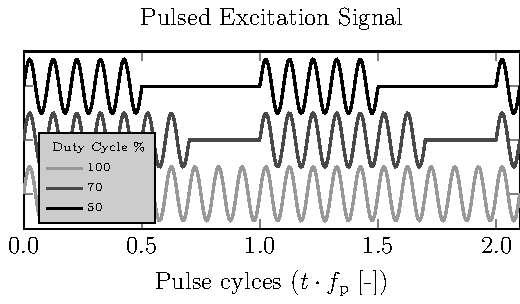
\includegraphics[]{External/duty-cycle.pdf}
  \caption{Schematic of pulsed acoustic excitation for three different duty 
      percentages (50, 70, and 100\%) and the relation $\fex=k\,\fp$ (here 
      $k=10$). 
      %\textbf{15 words}
  }\label{fig:PU-duty_cycle}
\end{figure}

The pulse frequencies $\fp$ we chose such that the fraction $\sfrac{\fex}{\fp}$ 
is an integer $k$. This means that per pulsing cycle 
($T_{\mathrm{p}}=\sfrac{1}{\fp}$) $k$ excitation periods 
$t_{0}=\sfrac{1}{\fex}$ are within $1\,T_{\mathrm{p}}$. As integer we set 
$k\in\{1'000, 5'000, 10'000\}$. The investigated duty percentages are 100\%, 
90\%, 80\%, 70\%, 60\%, and 50\%. The percentage value reflects the relative 
time the excitation is switched on within $1\,T_{\mathrm{p}}$ (see 
\cref{fig:PU-duty_cycle}). The BM with 100\% duty (\emph{always on}) is the 
baseline where the excitation is on for the entire BM. This BM is used for 
normalizing all other duty percentages at the same point $\Dy_{i}$ and pulse 
frequency $\fp$. The shortest pulse duration is for $k=1000$ and 50\% duty 
width. With these settings 500 \emph{on}-periods are followed by 500 
\emph{off}-periods before starting all over. The pressure amplitude build up is 
proportional to $\propto\left[ 1-\exp\left( \sfrac{-t}{\tau_{\mathrm{ARF}}} 
\right) \right]$ for this linear oscillating system. After 
$\sfrac{50}{\fex}\approx\SI{12.5}{\us}$ (50 excitation periods) the system is 
at 99.96\% of its steady-state amplitude. Although our system is subjected to 
two frequencies ($\fex$ and $\fp$) there are no influences on the pressure wave 
frequency because the build up is much faster than the shortest pulse.

All in all, compared to \cite{Goering2021} these three changes in the 
experimental settings are present: 1) 75 instead of 50 repetitions, 2) fixed 
$\Dz$ to \SI{0}{\um}, and 3) pulsed excitation signal.

%%%%%%%%%%%%%%%%%%%%%%%%%%%%%%%%%%%%%%%%%%%%%%%%%%%%%%%%%%%%%%%%%%%%%%%%%%%%%%
\section{Results and Discussion}

Before discussing our results, we want to emphasize that our experiments are 
very sensitive to external disturbances as well as the experimental condition. 
Because the whole experiment was newly initialised between the different $k$ 
values and, therefore, experimental conditions might change slightly, the 
results of different $k$ values are not fully quantitatively comparable.  
However, the trend for different $k$ values are nevertheless conclusive.

In \cref{fig:PU-duty-m05} the results of the BMs over time for $\Dy_{i}= 
\SI{-0.05}{\mm}$ are plotted. The figure consists of two columns (left for the 
ARF build up and right for the AS build up) and three rows for the three 
different pulsing frequencies $\fp$; in the 1\textsuperscript{st} row 
$\fp=\sfrac{\fex}{1'000}$, in the 2\textsuperscript{nd} row 
$\fp=\sfrac{\fex}{5'000}$, and in the 3\textsuperscript{rd} row 
$\fp=\sfrac{\fex}{10'000}$, respectively. For $\fp=\sfrac{\fex}{5'000}$ the 
data for the duty percentages of 70\%, 60\% and 50\% are not available. A data 
series with a duty percentage of 100\% has the same experimental settings as 
the data from \cite{Goering2021}. Hence, the results also show the same 
behavior: the initial build up of the ARF is significantly faster than the 
build up of AS. The data for $k=1000$ and 80\% duty width shows an unexpected 
behaviour because its magnitude is almost as strong as for 100\%. During the 
80\% BM series an unknown external disturbance caused a significant drop in the 
ambient room temperature (see also Fig. 5 in [supplemental material]). The 
measurement itself is not very sensitive to temperature fluctuations within 
\SI{1}{\degreeCelsius}. However, the OT is very sensitive to ambient noise. 
E.g, fast movement of a person in the room or careless opening or closing of 
the door can be detected by the OT. We attribute this outlayer of $k=1000$ and 
80\% to an external disturbance that also caused the significant temperature 
drop.

For the three different pulsing frequencies the time difference between the ARF 
and AS of the 100\% duty width measurements for reaching 50\% of the maximal 
value (horizontal dotted lines in \cref{fig:PU-duty-m05}) is $76-57=19[\cdot 
10^{3}\,\sfrac{t}{t_{0}}]$, $88-73=15[\cdot\,10^{3}\,\sfrac{t}{t_{0}}]$, and 
$94-78=16[\cdot\,10^{3}\,\sfrac{t}{t_{0}}]$ for $k=1'000, 5'000,\text{ and } 
10'000$, respectively. This 50\% criteria is the same measure we used in 
\cite{Goering2021} and, in addition, the time differences of the ARF and AS 
have the same magnitudes. However, the time at which the ARF is over 50\% of 
its maximal value is varying for the different $k$ values. Even though we 
limited the changes of the experimental settings between measurement series to 
a minimum, there are slight differences in the amplitude of the incident 
acoustic pressure field which cause these different values of the 50\% 
criteria. This is also the reason why for increasing values of $k$  the start 
time of the AS induced displacement is at a later point in time. In the 
[supplemental material] are two additional plots for $\Dy_{i} = \SI{-0.6}{\mm}$ 
and $\Dy_{i}= \SI{-0.4}{\mm}$ that show qualitatively and quantitatively the 
same behavior.

For all data series in all three plots, the normalized data is zero for 
$\sfrac{t}{t_{0}}=t\,\fex<0$ (gray shaded area). This is the time span where 
the US excitation is not switched on yet. Since the difference of the averaged 
on data subtracted from the averaged off data is shown and since both have the 
exact same protocol before the US is switched on, this behavior is expected and 
serves as quality control of a data series. A value close to zero after $t>0$ 
indicates that there is no difference in the movement of the particle along 
this direction for a switched on US and a switched off US. When the US is 
switched off, just gravity and the opposite directed buoyancy force are acting 
on the particle because the trapping laser is reduced to such a low laser power 
that the trap exerts negligible forces on the particle.

In addition, for a pulse frequency of $\fp=\sfrac{\fex}{10'000}$ and a duty 
cycle of 50\% the times where the US is switched on and off are visible in the 
data for the ARF (see bottom left plot in
\cref{fig:PU-duty-m05}). This movement resembles an upward going staircase and 
matches the times when the US is switched again on after one pulsing period 
$T_{\mathrm{p}}$. This is in line with the previous results from 
\cite{Goering2021} which showed that the ARF induced movement starts 
immediately as the US is switched on and stops as fast as it started when the 
US is switched off. No such staircase is visible for AS.

Additionally, for all positions $\Dy_{i}$ with a duty percentage of 50\% and a 
pulse frequency of $\fp=\sfrac{\fex}{10`000}$ the final measured value for AS 
is so low and close to zero that it might just be noise and no motion due to 
AS. On the other side, the ARF data for the same data series shows a clear 
displacement of the particle. The reason that we measure for all positions 
$\Dy_{i}$ with 50\% duty percentage and with a pulse frequency of 
$\fp=\sfrac{\fex}{1'000}$ an AS induced displacement is attributed to the 
slight differences in the experimental settings between BM series of different 
values of $k$.

\begin{figure*}[tbp]
  \centering
  % \tikzsetnextfilename{PU-duty-m05}
{
  \small
%%%%%%%
%%%%%%%
% READ TABLE
%%%%%%%
\pgfplotstableread{\relPath/10_Figures/TikZ/duty_fp_1000.dat}{\dataOne}
\pgfplotstableread{\relPath/10_Figures/TikZ/duty_fp_5000.dat}{\dataTwo}
\pgfplotstableread{\relPath/10_Figures/TikZ/duty_fp_10000.dat}{\dataThree}
%%%%%%%
% LINES FOR ALL GROUPPLOTS
%%%%%%%
\renewcommand{\tikzHelper}{
  \fill[fill=black!10!white] (axis cs:-80,0) rectangle (axis cs:0,1);

  \draw[dotted] (axis cs:0,0) -- (axis cs:0,1);
  \draw[dotted] (axis cs:50,0) -- (axis cs:50,1);
  \draw[dotted] (axis cs:100,0) -- (axis cs:100,1);
  \draw[dotted] (axis cs:-80,0.5) -- (axis cs:120,0.5);
  \draw[dotted] (axis cs:-80,0.5) -- (axis cs:120,0.5);
}


\begin{tikzpicture}
   \begin{groupplot}[%
       scale only axis,
       axis on top,
       group style={
         group size= 2 by 3,
         group name=plots,
         vertical sep=6pt,%
         horizontal sep=8pt},%
       height=40mm,%
       width=64mm,%
        xticklabel style={
          /pgf/number format/fixed,
          /pgf/number format/precision=2
        }]

%%%%%%
%%% PLOT (1,1)
%%%%%%

   \nextgroupplot[%
     legend cell align={left},
     legend style={
        fill=black!10!white,
        font=\tiny,
        at={(0.02,0.95)},
        anchor=north west,
        /tikz/column 2/.style={column sep=1pt,},
        legend columns=2,
      },
     xticklabels={,,},
     % title={$\DV_{y}\,|\,\Dy = \SI{-0.06}{\milli\meter}$},%
     title={ARF},%
     % title={Data for $y$-component},%
     ylabel={$\sfrac{\DV_{j}}{\DV_{100,\text{max}}}$ },
 ]

      \tikzHelper

      \addlegendimage{empty legend}
      \addlegendimage{empty legend}

      \addplot[style100] table[x=dt, y=DV_y_m05_100_m00] {\dataOne};
      \addplot[style90] table[x=dt, y=DV_y_m05_090_m00] {\dataOne};
      \addplot[style80] table[x=dt, y=DV_y_m05_080_m00] {\dataOne};
      \addplot[style70] table[x=dt, y=DV_y_m05_070_m00] {\dataOne};
      \addplot[style60] table[x=dt, y=DV_y_m05_060_m00] {\dataOne};
      \addplot[style50] table[x=dt, y=DV_y_m05_050_m00] {\dataOne};


      \addlegendentry{\hspace{-6mm}\textbf{Duty \%}}
      \addlegendentry{\textbf{\phantom{a}}}
      \addlegendentry{100};
      \addlegendentry{90};
      \addlegendentry{80};
      \addlegendentry{70};
      \addlegendentry{60};
      \addlegendentry{50};


%%%%%%
%%% PLOT (1,2)
%%%%%%

   \nextgroupplot[%
     xticklabels={,,},
     yticklabels={,,},
     % title={Data for $z$-component}]%
     title={AS},
   ]%

      \tikzHelper
      \draw[thick,|<->|] (axis cs:-80,0.25) -- (axis cs:0,0.25) node[midway, 
      above] {US off};

      \addplot[style100] table[x=dt, y=DV_z_m05_100_m00] {\dataOne};
      \addplot[style90] table[x=dt, y=DV_z_m05_090_m00] {\dataOne};
      \addplot[style80] table[x=dt, y=DV_z_m05_080_m00] {\dataOne};
      \addplot[style70] table[x=dt, y=DV_z_m05_070_m00] {\dataOne};
      \addplot[style60] table[x=dt, y=DV_z_m05_060_m00] {\dataOne};
      \addplot[style50] table[x=dt, y=DV_z_m05_050_m00] {\dataOne};

%%%%%%
%%% PLOT (2,1)
%%%%%%

   \nextgroupplot[%
     xticklabels={,,},
     ylabel={$\sfrac{\DV_{j}}{\DV_{100,\text{max}}}$ },
   ]

      \tikzHelper

      \addplot[style100] table[x=dt, y=DV_y_m05_100_m00] {\dataTwo};
      \addplot[style90] table[x=dt, y=DV_y_m05_090_m00] {\dataTwo};
      \addplot[style80] table[x=dt, y=DV_y_m05_080_m00] {\dataTwo};

%%%%%%
%%% PLOT (2,2)
%%%%%%

   \nextgroupplot[%
     xticklabels={,,},
     yticklabels={,,},
   ]

      \tikzHelper

      \addplot[style100] table[x=dt, y=DV_z_m05_100_m00] {\dataTwo};
      \addplot[style90] table[x=dt, y=DV_z_m05_090_m00] {\dataTwo};
      \addplot[style80] table[x=dt, y=DV_z_m05_080_m00] {\dataTwo};

%%%%%%
%%% PLOT (3,1)
%%%%%%

   \nextgroupplot[%
     ylabel={$\sfrac{\DV_{j}}{\DV_{100,\text{max}}}$ },
     xlabel={$10^{3}\,\sfrac{t}{t_{0}}$ },
   ]

      \tikzHelper

      \addplot[style100] table[x=dt, y=DV_y_m05_100_m00] {\dataThree};
      \addplot[style90] table[x=dt, y=DV_y_m05_090_m00] {\dataThree};
      \addplot[style80] table[x=dt, y=DV_y_m05_080_m00] {\dataThree};
      \addplot[style70] table[x=dt, y=DV_y_m05_070_m00] {\dataThree};
      \addplot[style60] table[x=dt, y=DV_y_m05_060_m00] {\dataThree};
      \addplot[style50] table[x=dt, y=DV_y_m05_050_m00] {\dataThree};

      \foreach \val/\index in 
      {50/0.104,60/0.138,70/0.161,80/0.205,90/0.241,100/0.277,110/0.310,120/0.36} {
        \edef\temp{\noexpand
        \draw[] (axis cs:\val, 0) -- (axis cs:\val,\index);
        }
        \temp}

%%%%%%
%%% PLOT (3,2)
%%%%%%

   \nextgroupplot[%
     yticklabels={,,},
     xlabel={$10^{3}\,\sfrac{t}{t_{0}}$ },
     % title={$\Dy = \SI{-0.04}{\milli\meter}$}
   ]

      \tikzHelper

      \addplot[style100] table[x=dt, y=DV_z_m05_100_m00] {\dataThree};
      \addplot[style90] table[x=dt, y=DV_z_m05_090_m00] {\dataThree};
      \addplot[style80] table[x=dt, y=DV_z_m05_080_m00] {\dataThree};
      \addplot[style70] table[x=dt, y=DV_z_m05_070_m00] {\dataThree};
      \addplot[style60] table[x=dt, y=DV_z_m05_060_m00] {\dataThree};
      \addplot[style50] table[x=dt, y=DV_z_m05_050_m00] {\dataThree};


  \end{groupplot}

%%%%%%
%%% TEXT NEXT TO PLOTS
%%%%%%
  \node[above] at ($(plots c1r1.north west)!0.5!(plots c2r1.north east)$) 
  [yshift=10mm] {$\Dy = \SI{-0.05}{\mm}$};

  \node[rotate=90] at (plots c2r2.east) [yshift=-5mm] {$k$};
  \node[rotate=90] at (plots c2r1.east) [yshift=-10mm] {1000};
  \node[rotate=90] at (plots c2r2.east) [yshift=-10mm] {5000};
  \node[rotate=90] at (plots c2r3.east) [yshift=-10mm] {10000};

\end{tikzpicture}
}

  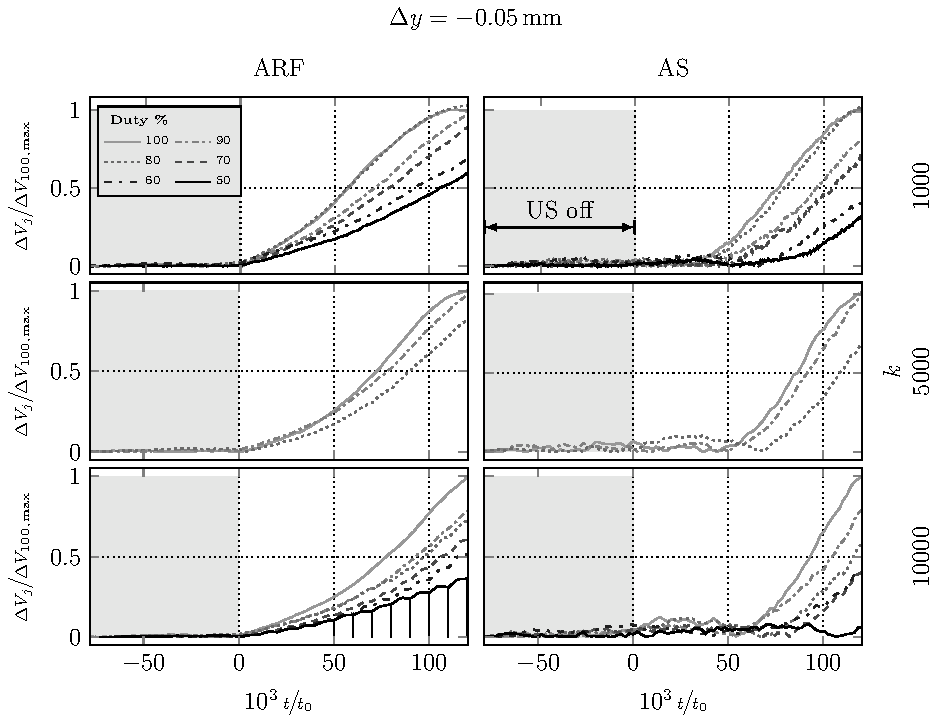
\includegraphics[]{External/duty-m05.pdf}
  \caption{Evolution of averaged voltage differences $\DV_{y}$ (left column; 
    ARF associated) and $\DV_{z}$ (right column; AS associated) for three 
    different pulsing frequencies $\fp$ and different duty percentages at 
    $\Dy=\SI{-0.5}{\mm}$. For the first row $\fp=\sfrac{\fex}{1'000}$, for the 
    second $\fp=\sfrac{\fex}{5'000}$, and for the last row 
    $\fp=\sfrac{\fex}{10'000}$. The data per plot is normalized to the maximal 
    amplitude of the data series with a duty percentage of 100\%. The vertical 
    solid lines in the bottom left plot mark the beginning of a new pulsing 
    cycle. 
    %\textbf{80 words}
}\label{fig:PU-duty-m05}
\end{figure*}

Even though, there are quantitative differences between the different pulse 
frequencies, qualitatively they have the same behavior. In all data series a 
reduced duty percentage is equivalent to a reduced and delayed build up of the 
ARF and AS. Since lower duty percentages lead to less energy in the system, 
this behavior is expected. However, the reduction of the AS build up is more 
than the reduction of the ARF. These different rates of reduction are more 
clearly visible in \cref{fig:PU-all-duty}.

There, the respective last normalized value of a data series of one specific 
duty percentage is plotted versus the duty percentage itself for each 
combination of BM point $\Dy_{i}$ and pulse frequency $\fp$. Each of these 
lines show a linear behavior over all duty percentages. However, the slope for 
the AS data is greater than for the ARF. This linear relation of the ARF for a 
one dimensional standing pressure field to the acoustic energy-density 
$E_{\mathrm{ac}}$ is in line with the theory
\begin{equation*}
  \FARF\propto E_{\mathrm{ac}} \propto p_{a}^{2}
\end{equation*}
where $p_{a}$ is the pressure of the acoustic field 
\cite{Gorkov1962,Bruus2012}. The same linear relation to the acoustic 
energy-density ($\FAS\propto E_{\mathrm{ac}}\propto p_{a}^{2}$) is 
theoretically valid for AS \cite{Bach2020} and also visible here. Nevertheless, 
the here depicted transient behavior of the ARF and AS suggests that the 
interrupted energy supply to the system causes an even further delay of the AS 
build up compared to the ARF build up. The generally lower values for the AS 
induced displacement and also the later start of the AS build up for 
$\fp=\sfrac{\fex}{10'000}$ compared to $\fp=\sfrac{\fex}{1'000}$ is attributed 
to the slight differences in the experimental settings and not a cause of the 
magnitude of $\fp$ itself.

\begin{figure*}[tbp]
  \centering
  % \tikzsetnextfilename{PU-avg-end-over-duty}
{
  \small
%%%%%%%
% READ TABLE
%%%%%%%
\pgfplotstableread{\relPath/10_Figures/TikZ/avg_end_over_duty.dat}{\data}
%%%%%%%
% LINES FOR ALL GROUPPLOTS
%%%%%%%
\begin{tikzpicture}
   \begin{groupplot}[%
       scale only axis,
       group style={
         group size= 2 by 1,
         group name=plots,
         vertical sep=4pt,%
         horizontal sep=20pt},%
       height=35mm,%
       width=64mm,%
       ymin=0, ymax=1.1,
        xticklabel style={
          /pgf/number format/fixed,
          /pgf/number format/precision=2
        }]

%%%%%%
%%% PLOT (1,1)
%%%%%%

   \nextgroupplot[%
      legend style={
        fill=lightgray!90!white,
        font=\footnotesize,
        at={(0.95,0.03)},
        legend columns=3,
        anchor=south east},
      legend cell align={left},
     title={ARF},%
     ylabel style={align=center},
     ylabel={{Normalized\\[-2.5mm] maximal amplitude}},
     xlabel={Duty width [\%]},
 ]

      \addlegendimage{empty legend}
      \addlegendimage{empty legend}
      \addlegendimage{empty legend}

      \addplot[style1000] table[x=duty, y=fp_1000_y] {\data};
      \addplot[style10000] table[x=duty, y=fp_10000_y] {\data};
      \addplot[style5000] table[x=duty, y=fp_5000_y] {\data};

      \addlegendentry{\phantom{a}}
      \addlegendentry{\hspace{-7mm}\textbf{$k$}}
      \addlegendentry{\phantom{a}}
      \addlegendentry{1000};
      \addlegendentry{5000};
      \addlegendentry{10000};


%%%%%%
%%% PLOT (1,2)
%%%%%%

   \nextgroupplot[%
     yticklabels={,,},
     xlabel={Duty width [\%]},
     title={AS},
   ]%

      \addplot[style1000] table[x=duty, y=fp_1000_z] {\data};
      \addplot[style5000] table[x=duty, y=fp_5000_z] {\data};
      \addplot[style10000] table[x=duty, y=fp_10000_z] {\data};

  \end{groupplot}

\end{tikzpicture}
}

  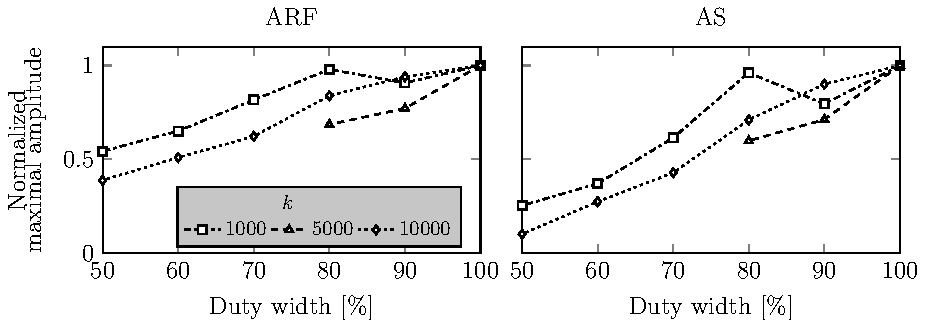
\includegraphics[]{External/avg-end-over-duty.pdf}
  \caption{Final normalized position at end of the build up measurement of 
  $\DV_{y}$ (left column; ARF associated) and $\DV_{z}$ (right column; AS 
  associated) over duty percentage for the three pulsing frequencies 
  $\fp=\sfrac{\fex}{k}$ and averaged over the three locations $\Dy_{i} =
\{\SI{-0.06}{\mm},\SI{-0.05}{\mm},\SI{-0.04}{\mm}\}$. The outlayer for $k=1000$ 
and 80\% duty width is attributed to an unknown external disturbance within the 
OT lab.}\label{fig:PU-all-duty}
\end{figure*}

%%%%%%%%%%%%%%%%%%%%%%%%%%%%%%%%%%%%%%%%%%%%%%%%%%%%%%%%%%%%%%%%%%%%%%%%%%%%%%
\section{Conclusion}
We extended our previous OT setup to measure the effects of a pulsed ultrasonic 
excitation of a microacoustofluidic system on the build up of the AS and the 
ARF, and also on the final position of a microparticle because of AS and the 
ARF. We varied the pulse frequency $\fp$ and duty width of the pulsed acoustic 
excitation to understand the effects of those parameters on the quantities of 
interest. In addition, we limited the difference of experimental settings 
between measurement series to a minimum for a valid comparison of the data. Our 
results show that the decrease in maximal displacement due to the ARF and the 
drag force from AS are both linear with respect to the applied duty percentage 
and more or less independent of the pulse frequency $\fp$. However, the 
decrease of AS with lower duty percentage is for all BMs faster than for the 
ARF. Even though our BM time span is limited to 120'000 acoustic excitation 
periods $\sfrac{1}{\fex}$ ($\approx$ \SI{96}{\ms}), we still manage to observe 
a significant level of streaming suppression, confirming the experimental 
results of Hoyos and Castro \cite{Castro2016,Hoyos2013}, and paving grounds for 
new theoretical studies that might improve our understanding of the AS build 
up.

%%%%%%%%%%%%%%%%%%%%%%%%%%%%%%%%%%%%%%%%%%%%%%%%%%%%%%%%%%%%%%%%%%%%%%%%%%%%%%

